%普通物理实验三林伟华老师要求的模板
%武汉大学物理科学与技术学院18级詹睿知
%改编自周澳同学转发的电子信息学院实验报告模板
\documentclass{whureport}
\usepackage{booktabs}%三线表
\usepackage{setspace}
\usepackage{stfloats}
\usepackage{graphicx}
\usepackage{datetime}
\usepackage{fancyhdr}
\usepackage{caption}
\captionsetup[table]{labelfont=bf,textfont=bf}
\usepackage{makecell}
\usepackage[breaklinks,colorlinks,linkcolor=black,
citecolor=black,urlcolor=black]{hyperref}
\newcommand{\major}{物理学}
<<<<<<< HEAD
\newcommand{\name}{袁俊}
\newcommand{\stuid}{2021300002080}
\newcommand{\Name}{Yuan Jun}
\newcommand{\loc}{None}
\newcommand{\course}{普通物理实验三}
\newcommand{\grades}{100}
\newcommand{\newtitle}{利用迈克尔逊干涉仪测量折射率}
\newcommand{\newtitlee}{Using Michelson interferometer to measure refractive index.}
=======
\newcommand{\name}{姓名}
\newcommand{\stuid}{学号}
\newcommand{\Name}{name}
\newcommand{\loc}{None}
\newcommand{\course}{普通物理实验三}
\newcommand{\grades}{100}
\newcommand{\newtitle}{实验名}
\newcommand{\etitle}{Title}
>>>>>>> 2da4d26b35807fdc082f05d652c9f8ded89414bd
\newcommand{\exptype}{None}
\usepackage{multicol}
%\usepackage{fontspec}
\setmainfont{Times New Roman}
\newfontfamily\sectionef{Times New Roman}
\newCJKfontfamily\sectioncf{kaishu}
\renewcommand\thesection{\arabic{section}}
\setlength{\parindent}{2em}
\lstset{language=Matlab}
\usepackage[algo2e,ruled,vlined]{algorithm2e}
\usepackage{ifthen}%这个宏包提供逻辑判断命令
\newboolean{first}%引入布尔变量
\setboolean{first}{true}%将布尔变量设置为true
\captionsetup{font={small}}
\fancypagestyle{maincontent}{
	\fancyhf{}  %清空页眉页脚设置
	\fancyhead[EL, OR]{\thepage}
	\fancyhead[EC]{\newtitle}
	\fancyhead[OC]{\newtitle}
	\renewcommand\headrulewidth{0pt}
}

\fancypagestyle{firstpage}{
	\fancyhf{}  
}

\newcommand{\makefirstpageheadrule}{
	\makebox[0pt][l]{\rule[0.55\baselineskip]{\headwidth}{0.2pt}}%上0.5pt,下0.2pt
	\rule[0.7\baselineskip]{\headwidth}{0.5pt}
}

\newcommand{\makeheadrule}{
	\rule[0.7\baselineskip]{\headwidth}{0.75pt}
}

\renewcommand{\headrule}{
	\ifthenelse{\boolean{first}}{\makeheadrule}
	{\makefirstpageheadrule}
}


\begin{document}
\pagestyle{maincontent} 
\bibliographystyle{plain}

\begin{center}
\zihao{-2} \textbf{\newtitle}\\
\zihao{7}~\\
\zihao{4} \kaishu \name \ \ (\stuid)\\
\zihao{5} \kaishu 武汉大学物理科学与技术学院,湖北省 武汉市 430072\\
\end{center}
\zihao{-5}\textbf{摘\quad 要:}
摘要内容。概括地陈述论文研究的目的、方法、结果、结论,要求200~300字。应排除本学科领域已成为常识的内容;不要把应在引言中出现的内容写入摘要,不引用参考文献;不要对论文内容作诠释和评论。不得简单重复题名中已有的信息。用第三人称,不使用“本文”、“作者”等作为主语。使用规范化的名词术语,新术语或尚无合适的汉文术语的,可用原文或译出后加括号注明。除了无法变通之外,一般不用数学公式和化学结构式,不出现插图、表格。缩略语、略称、代号,除了相邻专业的读者也能清楚理解的以外,在首次出现时必须加括号说明。结构严谨,表达简明,语义确切。\\
\zihao{-5}\textbf{关键词:}关键词1;关键词2;关键词3;关键词4
~\\
\begin{center}
<<<<<<< HEAD
	\zihao{3} \textbf{\newtitlee}\\
=======
	\zihao{3} \textbf{\etitle}\\
>>>>>>> 2da4d26b35807fdc082f05d652c9f8ded89414bd
	\zihao{5} \Name\quad (\stuid)\\
	\zihao{5} School of physical science and technology, Wuhan University, Wuhan, 430072, China
\end{center}

\zihao{5}\textbf{Abstract:}Purpose purpose purpose purpose purpose purpose purpose purpose purpose purpose purpose purpose purpose purpose purpose purpose purpose purpose purpose purpose purpose purpose purpose purpose purpose purpose purpose purpose purpose purpose purpose purpose. Method method method method method method method method method method method method method method method method method method. Result result result result result result result result result result result result result result result result result result result result result result result result result result result. Conclusion conclusion conclusion conclusion conclusion conclusion conclusion conclusion conclusion conclusion conclusion conclusion conclusion conclusion conclusion conclusion conclusion conclusion conclusion conclusion.

\zihao{5}\textbf{Keywords: }keyword1; keyword2; keyword3; keyword4

\begin{multicols}{2}
<<<<<<< HEAD
	\section{实验目的}
	\begin{enumerate}
		\item 目的1
		\item 目的2
		\item 目的3
	\end{enumerate}
	\section{实验仪器}
	\section{实验原理}
	\section{实验步骤}
	\subsection{数据表格}
	\subsection{数据处理}
	\subsection{误差分析}
=======
	引言内容。引言作为论文的开场白,应以简短的篇幅介绍论文的写作背景和目的,以及相关领域内前人所做的工作和研究概况,说明本研究与前人工作的关系,目前研究的热点、存在的问题及作者工作的意义。1、开门见山,不绕圈子。避免大篇幅地讲述历史渊源和立题研究过程。2、言简意赅,突出重点。不应过多叙述同行熟知的及教科书中的常识性内容,确有必要提及他人的研究成果和基本原理时,只需以引用参考文献的形势标出即可。在引言中提示本文的工作和观点时,意思应明确,语言应简练。3、引言的内容不要与摘要雷同,也不是摘要的注释。4、引言要简短,最好不要分段论述,不要插图、列表和数学公式。
	\section{量的书写规则}
	正文内容。正文、图表中的变量都要用斜体字母,对于矢量和张量使用黑斜体,只有pH采用正体;使用新标准规定的符号;量的符号为单个拉丁字母或希腊字母;不能把量符号作为纯数使用;不能把化学符号作为量符号使用,代表物质的符号表示成右下标,具体物质的符号及其状态等置于与主符号齐线的圆括号中\cite{snowflakes}。
	
	注意区分量的下标字母的正斜体:凡量符号和代表变动性数字及坐标轴的字母作下标,采用斜体字母。
	
	正文中引用参考文献的标注方法,在引用处对引用的文献,按它们在论著中出现的先后用阿拉伯数字连续排序,将序号置于方括号内,并视具体情况把序号作为上角标或作为语句的组成部分。
	\subsection{单位的书写规则}
	正文内容。单位符号无例外的采用正体字母\cite{jupyter}。注意区分单位符号的大小写:一般单位符号为小写体,来源于人名的单位符号首字母大写。体积单位升的符号为大写L。
	\subsubsection{表格的规范化}
	正文内容。表格的设计应该科学、明确、简洁,具有自明性。表格应采用三线表,项目栏不宜过繁,小表宽度小于7.5 cm,大表宽度为12~15cm 。
	
	正文内容。表格的设计应该科学、明确、简洁,具有自明性。表格应采用三线表,项目栏不宜过繁,小表宽度小于7.5 cm,大表宽度为12~15cm 。
	
	表必须有表序、表题。表中顶线与栏目线之间的部分叫项目栏,底线与栏目线之间的部分叫表身\cite{notebook}。表身中数字一般不带单位,百分数也不带百分号,应把单位符号和百分号等归并在栏目中。如果表中栏目中单位均相同,则可把共同的单位提出来标示在表格顶线上方的右端(不加“单位”二字)。表身中同一栏各行的数值应以个位(或小数点),且有效位数相同。上下左右相邻栏内的文字或数字相同时,应重复写出。
	
	\begin{table}[H]
		\centering
		\caption{表题}
		\small
		\begin{tabular}{ccccc}
			\Xhline{1.0pt}
			\makebox[0.1\textwidth][c]{xx}	&  \makebox[0.05\textwidth][c]{意义} &  \makebox[0.05\textwidth][c]{意义}&  \makebox[0.05\textwidth][c]{意义}&  \makebox[0.05\textwidth][c]{意义}\\ \Xhline{0.5pt}
			1&1&1&1&1\\
			2&2&2&2&2\\
			\Xhline{1.0pt}
		\end{tabular}
	\end{table}
	\section{图的规范化}
	\begin{figure}[H]
		\centering
		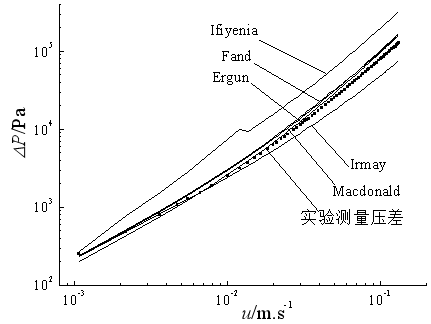
\includegraphics[width=.4\textwidth]{1.png}
		\caption{图题(杂志采用彩色印刷,图尽量也用彩色)}	
		\label{example}
	\end{figure}
	%注意,由于浮动体在multicols里是不允许的,我使用H强行把图放在这,在后续排版时注意图有没有跑
	
	\zihao{-5}正文内容。插图可用彩色图。小图宽度小于$7.8cm$,大图宽度为$12~15cm $。图必须有图序、图题。函数图只在靠近坐标线处残留一小段标值短线,其余部分省略。加注坐标所代表的量及单位(如t/s)。标值排印在坐标外侧,紧靠标值短线的地方;标值的有效数字为3位。图中量的意义要在正文中加以解释。若有图注,靠近放在图下部,图序、图题的上方。
	\section{数学符号和数学式的编排规范}
	正文内容。变量、变动附标及函数用斜体字母表示。点、线段及弧用斜体字母表示。在特定场合中视为常数的参数也用斜体字母表示。对具有特殊定义的函数和值不变的数学常数用正体字母表示\cite{physics}。具有特殊定义的算子也用正体字母表示。矩阵符号用大写的黑斜体字母表示,矩阵元素用白斜体字母表示。
	
	公式及公式中的符号说明尽量接排以节省版面。把带有复杂上角标的指数函数写成。公式的主体应排在同一水平线上;繁分式的主辅线要分清。长公式在运算符号后回行;长分式转行时,先将分母写成负幂指数的形式,然后转行;矩阵和行列式不能转行。矩阵元素包含式子时,每一列应以中心线上下对齐,行要左右排齐;元素为单个字母或数字时,每列应使正负号对齐。对角矩阵中对角元素所在的列应明显区分,不能上下重叠\cite{math}。
	
	简单的和常识性的运算公式和推导过程不要列写。
>>>>>>> 2da4d26b35807fdc082f05d652c9f8ded89414bd
	\section{结论}
	正文内容。结论不应是正文中各段小结的简单重复,它应以正文中的实验或考察得到的现象、数据的阐述分析为依据,完整、准确、简洁地指出以下内容:1)由对研究对象进行考察或实验得到的结果所揭示的原理及其普遍性;2)研究中有无发现例外或本论文尚难以解释和解决的问题;3)与先前发表过的研究工作的异同;4)本文在理论上和实用上的意义及价值;5)进一步深入研究本课题的建议。
	%\bibliography{article}
	\small
<<<<<<< HEAD
	\begin{thebibliography}{99}  

		\bibitem{ref1} 普物实验三 \ \  实验物理III\ \  -光学实验讲义-23\  下
	\end{thebibliography}
		
	%\bibliographystyle{ieee}
	%\bibliography{article}
\end{multicols}
=======
 \begin{thebibliography}{100}


\bibitem{ref1}普物实验三 \ \ \ \ 实验物理III\ \ \ \  -光学实验讲义-23下

\end{thebibliography}
	%\bibliographystyle{ieee}
	%\bibliography{article}
\end{multicols}

>>>>>>> 2da4d26b35807fdc082f05d652c9f8ded89414bd
\end{document}
